%%%%%%%%%%%%%%%%%%%%%%%%%%%%%%%%%%%%%%%%%%%%%%%%%%%%%%%%%%%%%%%%%%%%%%
% LaTeX Template: Curriculum Vitae
%
% Source: http://www.howtotex.com/
% Feel free to distribute this template, but please keep the
% referal to HowToTeX.com.
% Date: July 2011
% 
%%%%%%%%%%%%%%%%%%%%%%%%%%%%%%%%%%%%%%%%%%%%%%%%%%%%%%%%%%%%%%%%%%%%%%
\documentclass[paper=a4,fontsize=11pt]{scrartcl} % KOMA-article class
							
\usepackage[english]{babel}
\usepackage[utf8x]{inputenc}
\usepackage[protrusion=true,expansion=true]{microtype}
\usepackage{amsmath,amsfonts,amsthm}     % Math packages
\usepackage{graphicx}                    % Enable pdflatex
\usepackage[svgnames]{xcolor}            % Colors by their 'svgnames'
\usepackage{geometry}
	\textheight=700px                    % Saving trees ;-)
\usepackage{url}
\usepackage{wrapfig}

\frenchspacing              % Better looking spacings after periods
\pagestyle{empty}           % No pagenumbers/headers/footers

%%% Custom sectioning (sectsty package)
%%% ------------------------------------------------------------
\usepackage{sectsty}

\sectionfont{%			            % Change font of \section command
	\usefont{OT1}{phv}{b}{n}%		% bch-b-n: CharterBT-Bold font
	\sectionrule{0pt}{0pt}{-5pt}{3pt}}

%%% Macros
%%% ------------------------------------------------------------
\newlength{\spacebox}
\settowidth{\spacebox}{8888888888}			% Box to align text
\newcommand{\sepspace}{\vspace*{1em}}		% Vertical space macro

\newcommand{\MyName}[1]{ % Name
		\Huge \usefont{OT1}{phv}{b}{n} \hfill #1
		\par \normalsize \normalfont}
		
\newcommand{\MySlogan}[1]{ % Slogan (optional)
		\large \usefont{OT1}{phv}{m}{n}\hfill \textit{#1}
		\par \normalsize \normalfont}

\newcommand{\NewPart}[1]{\section*{\uppercase{#1}}}

\newcommand{\PersonalEntry}[2]{
		\noindent\hangindent=2em\hangafter=0 % Indentation
		\parbox{\spacebox}{        % Box to align text
		\textit{#1}}		       % Entry name (birth, address, etc.)
		\hspace{1.5em} #2 \par}    % Entry value

\newcommand{\SkillsEntry}[2]{      % Same as \PersonalEntry
		\noindent\hangindent=2em\hangafter=0 % Indentation
		\parbox{\spacebox}{        % Box to align text
		\textit{#1}}			   % Entry name (birth, address, etc.)
		\hspace{1.5em} #2 \par}    % Entry value	
		
\newcommand{\EducationEntry}[4]{
		\noindent \textbf{#1} \hfill      % Study
		\colorbox{Black}{%
			\parbox{6em}{%
			\hfill\color{White}#2}} \par  % Duration
		\noindent \textit{#3} \par        % School
		\noindent\hangindent=2em\hangafter=0 \small #4 % Description
		\normalsize \par}

\newcommand{\WorkEntry}[4]{				  % Same as \EducationEntry
		\noindent \textbf{#1} \hfill      % Jobname
		\colorbox{Black}{\color{White}#2} \par  % Duration
		\noindent \textit{#3} \par              % Company
		\noindent\hangindent=2em\hangafter=0 \small #4 % Description
		\normalsize \par}

%%% Begin Document
%%% ------------------------------------------------------------

\begin{document}

\begin{wrapfigure}{l}{0.5\textwidth}
	\vspace*{-2em}
        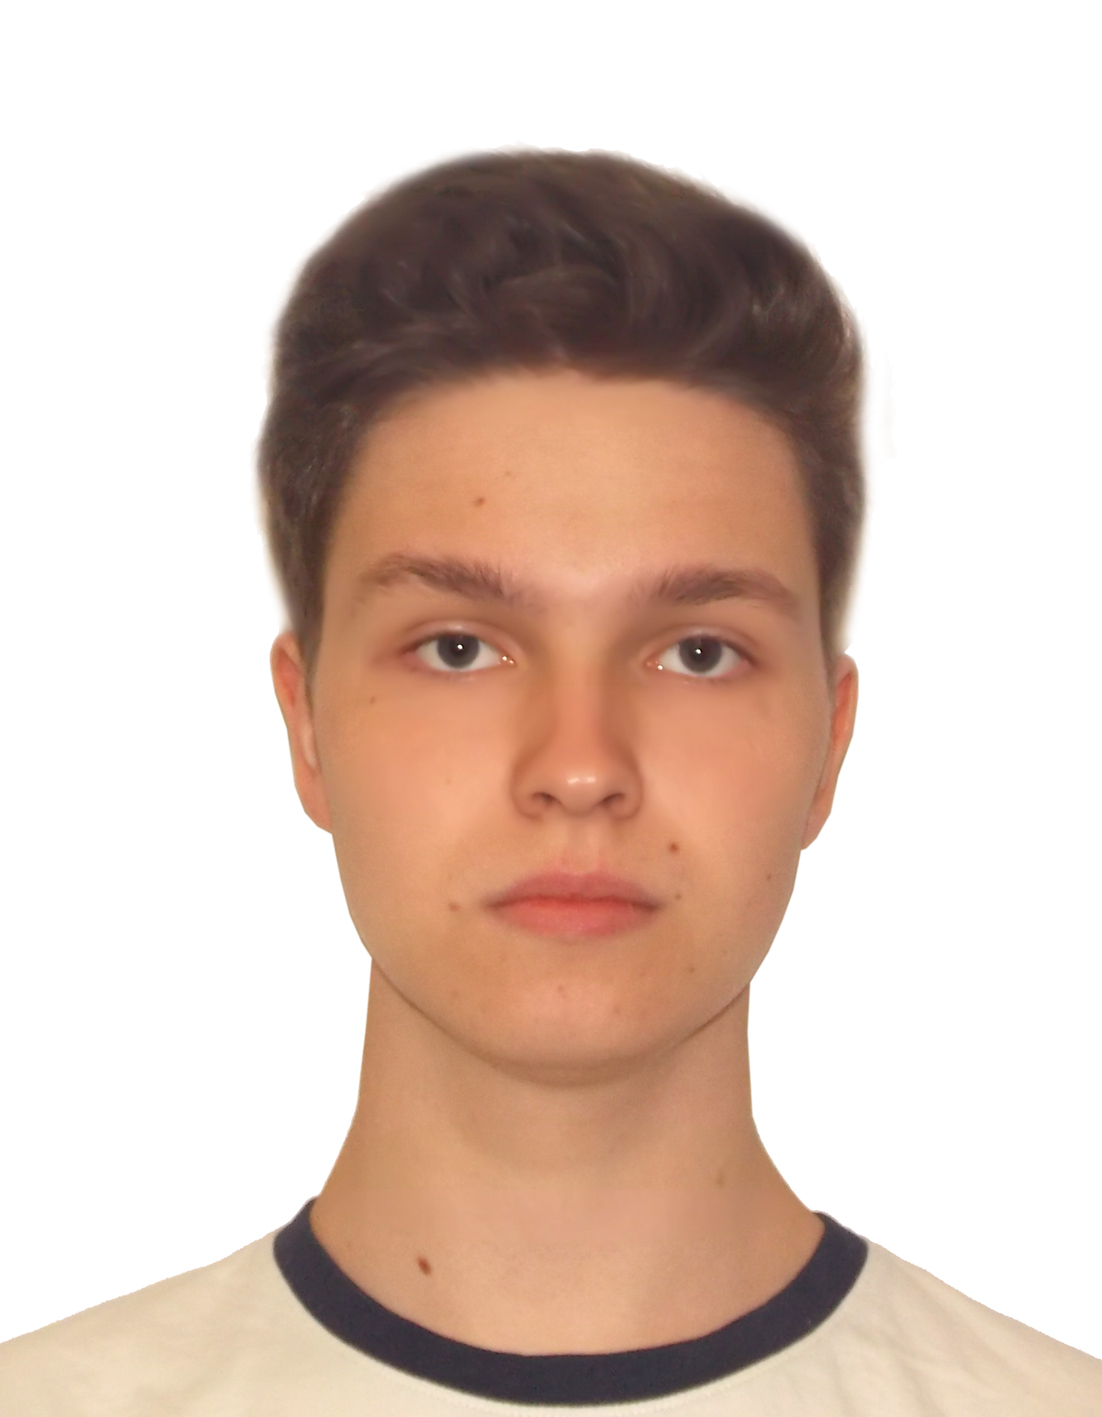
\includegraphics[width=0.15\textwidth]{photo}
\end{wrapfigure}

\MyName{MIKHAIL}
\MyName{GORELYI}

\sepspace

%%% Personal details
%%% ------------------------------------------------------------
\NewPart{Personal details}{}

\PersonalEntry{Birth}{March 03, 2002}
\PersonalEntry{Address}{Russia, Moscow 109125}
\PersonalEntry{Phone}{+7(982)724-31-64}
\PersonalEntry{E-mail}{\url{gorelyy02@gmail.com}}

%%% Education
%%% ------------------------------------------------------------
\NewPart{Education}{}

\EducationEntry{National Research University Higher School of Economics, Moscow }{2020-present}{Faculty of Computer Science\\Applied Mathematics and Informatics\\GPA: 8.63}

%%% Work experience
%%% ------------------------------------------------------------
\NewPart{INTERNSHIPS}{}

\WorkEntry{Research Trainee}{October'21-present}{NRU HSE, Laboratory of Complex Systems Modeling and Control}{Title : Relational inductive biases, deep learning, and graph networks\\Supervision : Under Dr. Malay Bhattacharyya, ISI, Kolkata\\About : Analyzing the neural networks to operate on graphs.}

%%% project
%%% ------------------------------------------------------------
\NewPart{Projects}{}

\WorkEntry{M.Tech Project}{July'18-June'19}{Direct Torque Control of Induction Motor}{Supervision : Under Dr. N K Swami Naidu, IIT BHU, Varanasi\\We have developed a Network-On-Chip simulator, Noxim. Our main objective was \\to develop a simulator that can perform all types of functionalities in a single platform.}
\sepspace


\WorkEntry{Personal Project}{December'21-present}{Supervision : Under Dr. Prasun Ghosal, IIEST, Shibpur\\Online Compiler and data storage}{I am working on a website from where anyone can take help for their coding, they can upload their codes
there, they can compile codes. If anyone wants to ask for help for particular purpose they can post their
problem statement there.}

%%% Skills
%%% ------------------------------------------------------------
\NewPart{Skills}{}

\SkillsEntry{Languages}{Russian (mother tongue)}
\SkillsEntry{}{English (advanced)}
\sepspace

\SkillsEntry{Programming Languages}{\textsc{C/C++},\textsc{Python}}
\sepspace


\SkillsEntry{Subjects}{\textsc{Advanced C++}, \textsc{Linear Algebra}}
\SkillsEntry{}{\textsc{Algorithms and Data Structures}}
\SkillsEntry{}{\textsc{Discrete Mathematics}, \textsc{Calculus}, \textsc{Algebra}}
\SkillsEntry{}{\textsc{Computer Architecture and Operating Systems}}


%%% References
%%% ------------------------------------------------------------
\NewPart{Extra Curricular Activities}{}
1. Swimming
\\
2. Playing the guitar
\end{document}
